\documentclass[a4paper]{scrreprt}


%% Language and font encodings
\usepackage[german]{babel}
\setcounter{secnumdepth}{3} 
\setcounter{tocdepth}{3} 
\usepackage[utf8x]{inputenc}
\usepackage[T1]{fontenc}
\usepackage{courier}

%% Sets page size and margins
\usepackage[a4paper,top=3cm,bottom=2cm,left=3cm,right=3cm,marginparwidth=1.75cm]{geometry}

%% Useful packages
\usepackage{amsmath}
\usepackage{graphicx}
\usepackage[colorinlistoftodos]{todonotes}
\usepackage[colorlinks=true, allcolors=blue]{hyperref}

\title{Entwurfsdokument}
\author{   Yunjia Chen, Jasmin Jat, Min Hye Park, Alina Shah, Lisa Wang}

\begin{document}
\maketitle
\tableofcontents 
\newpage
\chapter{Einleitung}

\chapter{Grobentwurf}
	\section{Entwurfsentscheidungen}
    	\subsection{Activity}
        Unsere App setzt sich aus 15 Activites zusammen. Die Activities stellen die Benutzerschnittstelle unserer App dar und kümmern sich um die Interaktionen mit unserer Benutzeroberfläche. In jeder Activity-Klasse befinden sich selbstverständlich die üblichen Methoden eines Activity-Lifecycles: onCreate() zum Erstellen, onStart() zum Starten, onPause() zum Pausieren , onResume() zum Fortsetzen, onStop() zum Stoppen und onDestroy() zum Zerstören der Activity.
        
        
\newpage

\chapter{Feinentwurf}
	\section{Klassen des Clients}
	\subsection{package kit.edu.pse.fridget.client.activity}
\begin{figure}[H]
	       \centering
	       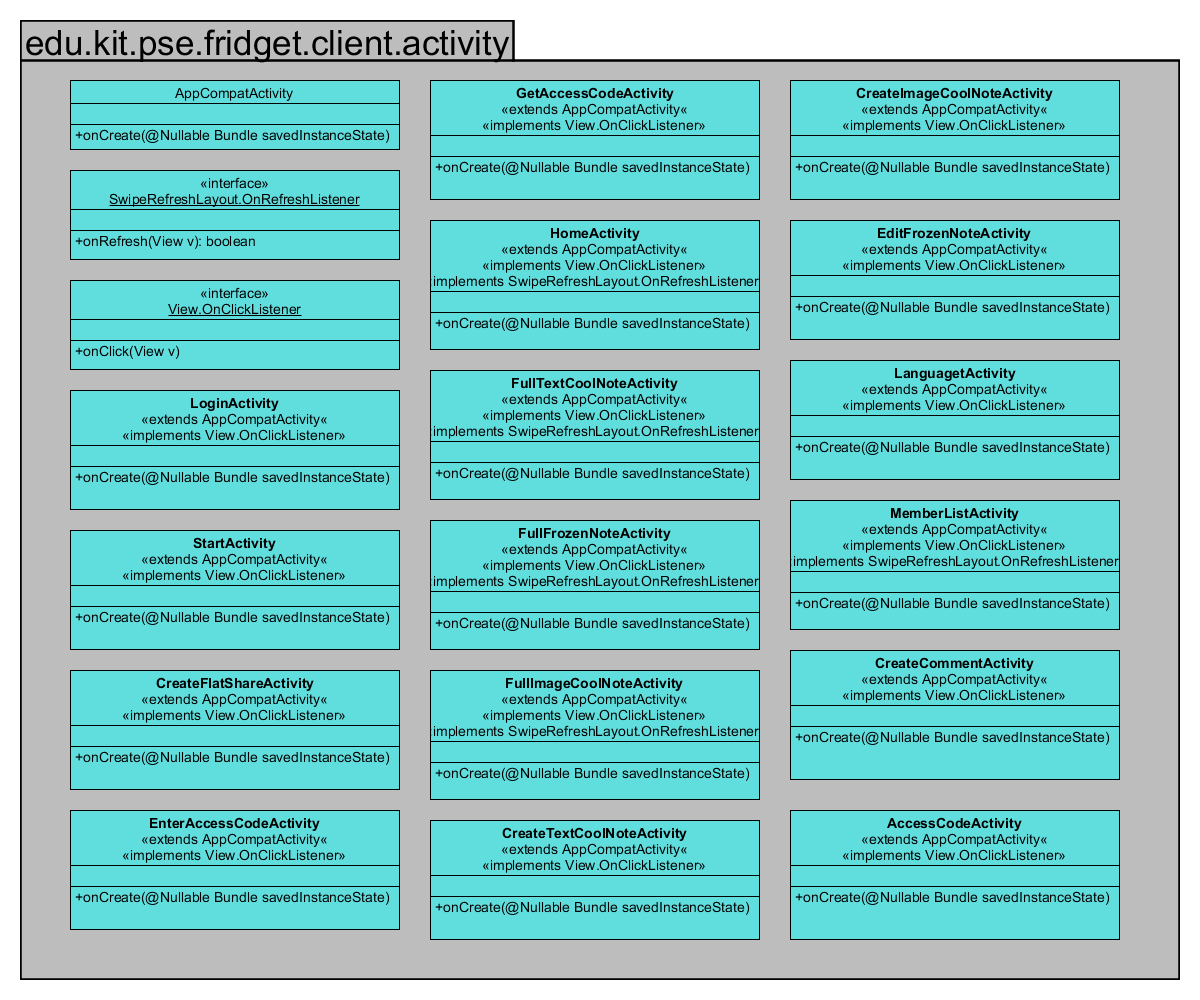
\includegraphics[scale = .35]{klassendiagramm_activity.png}
	       \caption{Klassen der Activities}
	      \end{figure}
\subsubsection{\texttt{public class AppCompatActivity}}

Unsere App setzt sich aus 16 Activites zusammen.\\

	\textbf{Beschreibung} \\
	\textit{Basisklasse für alle Activities} \\

	\textbf{Methoden}
	\begin{itemize}
		\item{\texttt{public void onCreate(@Nullable Bundle savedInstanceState)}}\\
	\textit{Hier wird das Layout der Activity erstellt.}\\
	\end{itemize}

	\textbf{Parameter}
	\begin{itemize}
		\item\texttt{Bundle savedInstanceState}\\ 
	\textit{Die zuvor gespeicherte Instanz der Activity, die wieder hergestellt zwird, sonst NULL}\\
	\end{itemize}

\subsubsection{\texttt{public static interface View.OnClickListener}}

	\textbf{Beschreibung} \\
	\textit{Schnittstelle dafür, wenn auf die View geklickt wird.klickt wird.}\\

	\textbf{Methoden}
	\begin{itemize}
	\item{\texttt{public void onClick(View v)}}\\
	\textit{Aufruf bei einen Klick auf ein Element.}\\
	\end{itemize}

	\textbf{Parameter}
	\begin{itemize}
	\item\texttt{View v}\\
	\textit{Die angeklickte View}\\
	\end{itemize} 

\subsubsection{\texttt{public static interface SwipeRefreshLayout.OnRefreshListener}}

	\textbf{Beschreibung} \\
	\textit{Schnittstelle dafür, wenn durch Hinunter-Swipen eine Aktualisierung ausgeführt werden soll} \\

	\textbf{Methoden}
	\begin{itemize}
		\item\texttt{{public boolean onRefresh()}}\\
	\textit{Aufruf beim Hinunter-Swipen zum Aktualisieren}\\
	\end{itemize}       

\subsubsection{\texttt{public class LoginActivity extends AppCompatActivity implements View.OnClickListener}}

	\textbf{Beschreibung} \\
	\textit{Diese Klasse zeigt den Login mit dem Google-Account. Man kann seinen Google-Account-Daten eingeben und sich anmelden.} \\

	\textbf{Methoden}
	\begin{itemize}
		\item\texttt{{public void onCreate(@Nullable Bundle savedInstanceState)}}\\
	\textit{Hier wird das Layout der Activity erstellt.}\\
	\end{itemize}

	\textbf{Parameter}
	\begin{itemize}
		\item\texttt{Bundle savedInstanceState}\\ 
	\textit{Die zuvor gespeicherte Instanz der Activity, die wieder hergestellt zwird, sonst NULL}\\
	\end{itemize}

\subsubsection{\texttt{public class StartActivity extends AppCompatActivity implements View.OnClickListener}}

	\textbf{Beschreibung} \\
	\textit{Diese Klasse zeigt den Startbildschirm mit dem App-Logo und zwei Buttons: Ein Button zum Erstellen einer WG und einer zum Eingeben eines Zugangscodes.} \\

	\textbf{Methoden}
	\begin{itemize}
		\item\texttt{{public void onCreate(@Nullable Bundle savedInstanceState)}}\\
	\textit{Hier wird das Layout der Activity erstellt.}\\
	\end{itemize}

	\textbf{Parameter}
	\begin{itemize}
		\item\texttt{Bundle savedInstanceState}\\ 
	\textit{Die zuvor gespeicherte Instanz der Activity, die wieder hergestellt zwird, sonst NULL}\\
	\end{itemize}       

\subsubsection{\texttt{public class CreateFlatshareActivity extends AppCompatActivity implements View.OnClickListener}}

	\textbf{Beschreibung} \\
	\textit{In dieser Klasse kann man der WG einen Namen geben und kann mithilfe eines Buttons zur HomeActivity gelangen.} \\

	\textbf{Methoden}
	\begin{itemize}
		\item\texttt{{public void onCreate(@Nullable Bundle savedInstanceState)}}\\
	\textit{Hier wird das Layout der Activity erstellt.}\\
	\end{itemize}

	\textbf{Parameter}
	\begin{itemize}
		\item\texttt{Bundle savedInstanceState}\\ 
	\textit{Die zuvor gespeicherte Instanz der Activity, die wieder hergestellt zwird, sonst NULL}\\
	\end{itemize}      

\subsubsection{\texttt{public class GetAccessCodeActivity extends AppCompatActivity implements View.OnClickListener}}

	\textbf{Beschreibung} \\
	\textit{In dieser Klasse kriegt man den Zugangscode und kann mithilfe eines Buttons zur HomeActivity gelangen.} \\

	\textbf{Methoden}
	\begin{itemize}
		\item\texttt{{public void onCreate(@Nullable Bundle savedInstanceState)}}\\
	\textit{Hier wird das Layout der Activity erstellt.}\\
	\end{itemize}

	\textbf{Parameter}
	\begin{itemize}
		\item\texttt{Bundle savedInstanceState}\\  
	\textit{Die zuvor gespeicherte Instanz der Activity, die wieder hergestellt zwird, sonst NULL}\\
	\end{itemize}  

\subsubsection{\texttt{public class EnterAccessCodeActivity extends AppCompatActivity implements View.OnClickListener}}

	\textbf{Beschreibung} \\
	\textit{In dieser Klasse kann man den Zugangscode eingeben und kann mithilfe eines Buttons zur HomeActivity gelangen.} \\

	\textbf{Methoden}
	\begin{itemize}
		\item\texttt{{public void onCreate(@Nullable Bundle savedInstanceState)}}\\
	\textit{Hier wird das Layout der Activity erstellt.}\\
	\end{itemize}

	\textbf{Parameter}
	\begin{itemize}
		\item\texttt{Bundle savedInstanceState}\\ 
	\textit{Die zuvor gespeicherte Instanz der Activity, die wieder hergestellt zwird, sonst NULL}\\
	\end{itemize} 

\subsubsection{\texttt{public class HomeActivity extends AppCompatActivity implements View.OnClickListener implements SwipeRefreshLayout.OnRefreshListener}}

	\textbf{Beschreibung} \\
	\textit{Diese Klasse zeigt das View der WG-Pinnwand, man sieht die Notes mit Überschrift und Magnet und einige Buttons. Drei Frozen Notes sind von Anfang an enthalten. Frozen Notes haben immer einen schwarzen Magneten.} \\

	\textbf{Methoden}
	\begin{itemize}
		\item\texttt{{public void onCreate(@Nullable Bundle savedInstanceState)}}\\
	\textit{Hier wird das Layout der Activity erstellt.}\\
	\end{itemize}

	\textbf{Parameter}
	\begin{itemize}
		\item\texttt{Bundle savedInstanceState}\\  
	\textit{Die zuvor gespeicherte Instanz der Activity, die wieder hergestellt zwird, sonst NULL}\\
	\end{itemize} 

\subsubsection{\texttt{public class FullTextCoolNoteActivity extends AppCompatActivity implements View.OnClickListener implements SwipeRefreshLayout.OnRefreshListener}}

	\textbf{Beschreibung} \\
	\textit{Diese Klasse zeigt eine Großansicht einer Text-Cool-Note mit zugehörigem Magneten, Erstelldatum, Tags, Titel, Inhalt, Lesebestätigungen und Kommentaren. Der @All-Tag ist immer da, wenn keine Tags spezifiziert werden. Es stehen wieder einige Buttons zur Interaktion zu Verfügung.} \\

	\textbf{Methoden}
	\begin{itemize}
		\item\texttt{{public void onCreate(@Nullable Bundle savedInstanceState)}}\\
	\textit{Hier wird das Layout der Activity erstellt.}\\
	\end{itemize}

	\textbf{Parameter}
	\begin{itemize}
		\item\texttt{Bundle savedInstanceState}\\ 
	\textit{Die zuvor gespeicherte Instanz der Activity, die wieder hergestellt zwird, sonst NULL}\\
	\end{itemize} 

\subsubsection{\texttt{public class FullFrozenNoteActivity extends AppCompatActivity implements View.OnClickListener implements SwipeRefreshLayout.OnRefreshListener}}

	\textbf{Beschreibung} \\
	\textit{Diese Klasse zeigt eine Großansicht einer Frozen Note mit zugehörigem schwarzen Magneten, Titel und Inhalt. Es stehen wieder einige Buttons zur Interaktion zu Verfügung.} \\

	\textbf{Methoden}
	\begin{itemize}
		\item\texttt{{public void onCreate(@Nullable Bundle savedInstanceState)}}\\
	\textit{Hier wird das Layout der Activity erstellt.}\\
	\end{itemize}

	\textbf{Parameter}
	\begin{itemize}
		\item\texttt{Bundle savedInstanceState}\\ 
	\textit{Die zuvor gespeicherte Instanz der Activity, die wieder hergestellt zwird, sonst NULL}\\
	\end{itemize} 

\subsubsection{\texttt{public class FullImageCoolNoteActivity extends AppCompatActivity implements View.OnClickListener implements SwipeRefreshLayout.OnRefreshListener}}

	\textbf{Beschreibung} \\
	\textit{Diese Klasse zeigt eine Großansicht einer Bild-Cool-Note mit zugehörigem Magneten, Erstelldatum, Tags, Titel, Inhalt, Lesebestätigungen und Kommentaren. Der @All-Tag ist immer da, wenn keine Tags spezifiziert werden. Es stehen wieder einige Buttons zur Interaktion zu Verfügung.} \\

	\textbf{Methoden}
	\begin{itemize}
		\item\texttt{{public void onCreate(@Nullable Bundle savedInstanceState)}}\\
	\textit{Hier wird das Layout der Activity erstellt.}\\
	\end{itemize}

	\textbf{Parameter}
	\begin{itemize}
		\item\texttt{Bundle savedInstanceState}\\ 
	\textit{Die zuvor gespeicherte Instanz der Activity, die wieder hergestellt zwird, sonst NULL}\\
	\end{itemize} 

\subsubsection{\texttt{public class CreateTextCoolNoteActivity extends AppCompatActivity implements View.OnClickListener}}

	\textbf{Beschreibung} \\
	\textit{Diese Klasse zeigt das View für die Erstellung einer Text-Cool-Note. Dieses View wird auch für die Kommentar-Funktion benutzt, nur, dass man keinen Titel schreiben und keine Wichtigkeit auswählen kann. Das View öffnet sich auch, wenn man eine Frozen Note editieren will, wobei die Wichtigkeit wieder nicht auswählbar ist.} \\

	\textbf{Methoden}
	\begin{itemize}
		\item\texttt{{public void onCreate(@Nullable Bundle savedInstanceState)}}\\
	\textit{Hier wird das Layout der Activity erstellt.}\\
	\end{itemize}

	\textbf{Parameter}
	\begin{itemize}
		\item\texttt{Bundle savedInstanceState}\\  
	\textit{Die zuvor gespeicherte Instanz der Activity, die wieder hergestellt zwird, sonst NULL}\\
	\end{itemize} 


\subsubsection{\texttt{public class CreateImageCoolNoteActivity extends AppCompatActivity implements View.OnClickListener}}

	\textbf{Beschreibung} \\
	\textit{Diese Klasse zeigt das View für die Erstellung einer Bild-Cool-Note.} \\

	\textbf{Methoden}
	\begin{itemize}
		\item\texttt{{public void onCreate(@Nullable Bundle savedInstanceState)}}\\
	\textit{Hier wird das Layout der Activity erstellt.}\\
	\end{itemize}

	\textbf{Parameter}
	\begin{itemize}
		\item\texttt{Bundle savedInstanceState}\\ 
	\textit{Die zuvor gespeicherte Instanz der Activity, die wieder hergestellt zwird, sonst NULL}\\
	\end{itemize} 

\subsubsection{\texttt{public class CreateCommentActivity extends AppCompatActivity implements View.OnClickListener}}

	\textbf{Beschreibung} \\
	\textit{Diese Klasse zeigt das View für die Erstellung eines Kommentars.} \\

	\textbf{Methoden}
	\begin{itemize}
		\item\texttt{{public void onCreate(@Nullable Bundle savedInstanceState)}}\\
	\textit{Hier wird das Layout der Activity erstellt.}\\
	\end{itemize}

	\textbf{Parameter}
	\begin{itemize}
		\item\texttt{Bundle savedInstanceState}\\  
	\textit{Die zuvor gespeicherte Instanz der Activity, die wieder hergestellt zwird, sonst NULL}\\
	\end{itemize} 


\subsubsection{\texttt{public class EditFrozenNoteActivity extends AppCompatActivity implements View.OnClickListener}}

	\textbf{Beschreibung} \\
	\textit{Diese Klasse zeigt das View für die Bearbeitung einer Frozen Note.} \\

	\textbf{Methoden}
	\begin{itemize}
		\item\texttt{{public void onCreate(@Nullable Bundle savedInstanceState)}}\\
	\textit{Hier wird das Layout der Activity erstellt.}\\
	\end{itemize}

	\textbf{Parameter}
	\begin{itemize}
		\item\texttt{Bundle savedInstanceState}\\ 
	\textit{Die zuvor gespeicherte Instanz der Activity, die wieder hergestellt zwird, sonst NULL}\\
	\end{itemize} 

\subsubsection{\texttt{public class MemberListActivity extends AppCompatActivity implements View.OnClickListener implements SwipeRefreshLayout.OnRefreshListener}}

	\textbf{Beschreibung} \\
	\textit{Diese Klasse zeigt das View zum Einsehen der aktuellen Mitglieder mit
mit zugehörigem Magneten.} \\

	\textbf{Methoden}
	\begin{itemize}
		\item\texttt{{public void onCreate(@Nullable Bundle savedInstanceState)}}\\
	\textit{Hier wird das Layout der Activity erstellt.}\\
	\end{itemize}

	\textbf{Parameter}
	\begin{itemize}
		\item\texttt{Bundle savedInstanceState}\\  
	\textit{Die zuvor gespeicherte Instanz der Activity, die wieder hergestellt zwird, sonst NULL}\\
	\end{itemize} 

\subsubsection{\texttt{public class LanguageActivity extends AppCompatActivity implements View.OnClickListener}}

	\textbf{Beschreibung} \\
	\textit{Diese Klasse zeigt das View zum Einstellen der App-Sprache.} \\

	\textbf{Methoden}
	\begin{itemize}
		\item\texttt{{public void onCreate(@Nullable Bundle savedInstanceState)}}\\
	\textit{Hier wird das Layout der Activity erstellt.}\\
	\end{itemize}

	\textbf{Parameter}
	\begin{itemize}
		\item\texttt{Bundle savedInstanceState}\\  
	\textit{Die zuvor gespeicherte Instanz der Activity, die wieder hergestellt zwird, sonst NULL}\\
	\end{itemize} 

\subsubsection{\texttt{public class AccessCodeActivity extends AppCompatActivity implements View.OnClickListener}}

\textbf{Beschreibung} \\
\textit{Diese Klasse zeigt das View zum Erstellen eines neuen Zugangscodes.} \\

\textbf{Methoden}
\begin{itemize}
	\item\texttt{{public void onCreate(@Nullable Bundle savedInstanceState)}}\\
	\textit{Hier wird das Layout der Activity erstellt.}\\
\end{itemize}

\textbf{Parameter}
\begin{itemize}
	\item\texttt{Bundle savedInstanceState}\\  
	\textit{Die zuvor gespeicherte Instanz der Activity, die wieder hergestellt zwird, sonst NULL}\\
\end{itemize} 

\newpage


    \section{Klassen des Servers}
    %\documentclass[a4paper]{scrreprt}

%\usepackage[german]{babel}
%\usepackage[utf8]{inputenc}
%\usepackage[T1]{fontenc}
%\usepackage{ae}
%\usepackage{tocbasic}

%\begin{document}
    \section{Package edu.kit.pse.fridget.server.controllers}
    \subsection{\texttt{Class AccessCodeController}}
    \textbf{Beschreibung} \\
    \textit{Controller für Zugangscode}
    \subsubsection{Konstruktor}
    \texttt{public AccessCodeController(AccessCodeService service)}
    \subsubsection{Methoden}
    \begin{itemize}
    	\item{\texttt{public ResponseEntity<AccessCode> generateAccessCode(GenerateAccessCodeCommand generateAccessCodeCommand)}}
    	
    	\textit{Generiert einen Zugangscode für eine WG.}
    	
    	\textbf{Parameter} \\
    	generateAccessCodeCommand WG-ID
    	
    	\textbf{Rückgabewert} \\
    	Generierter Zugangscode als ResponseEntity
    \end{itemize}
    \subsection{\texttt{Class CommentController}}
    \textbf{Beschreibung} \\
    \textit{Controller für Kommentar}
    \subsubsection{Konstruktor}
    \texttt{public CommentController(CommentService service)}
    \subsubsection{Methoden}
    \begin{itemize}
    	\item{\texttt{public ResponseEntity<List<Comment$>>$ getAllComments(String coolNoteId)}}
    	
    	\textit{Findet alle Kommentare zu einer Cool Note.}
    	
    	\textbf{Parameter} \\
    	coolNoteId CoolNote-ID
    	
    	\textbf{Rückgabewert} \\
    	Liste von gefundenen Kommentaren als ResponseEntity        \item{\texttt{public ResponseEntity<Comment> saveComment(Comment comment)}}
    	
    	\textit{Speichert einen Kommentar.}
    	
    	\textbf{Parameter} \\
    	comment Kommentar zum speichern
    	
    	\textbf{Rückgabewert} \\
    	Gespeicherter Kommentar als ResponseEntity        \item{\texttt{public ResponseEntity<Void> deleteComment(String id)}}
    	
    	\textit{Löscht einen Kommentar.}
    	
    	\textbf{Parameter} \\
    	id Kommentar-ID
    	
    	\textbf{Rückgabewert} \\
    	Leere ResponseEntity
    \end{itemize}
    \subsection{\texttt{Class CoolNoteController}}
    \textbf{Beschreibung} \\
    \textit{Controller für Cool Note}
    \subsubsection{Konstruktor}
    \texttt{public CoolNoteController(CoolNoteService coolNoteService, TaggedUserService taggedUserService)}
    \subsubsection{Methoden}
    \begin{itemize}
    	\item{\texttt{public ResponseEntity<List<CoolNoteWithTaggedUsersRepresentation$>>$ getAllCoolNotes(String flatshareId)}}
    	
    	\textit{Findet alle Cool Notes mit getaggten Benutzern in einer WG.}
    	
    	\textbf{Parameter} \\
    	flatshareId WG-ID
    	
    	\textbf{Rückgabewert} \\
    	Liste von gefundenen CoolNote mit ID von getaggten Benutzern als ResponseEntity        \item{\texttt{public ResponseEntity<CoolNoteWithTaggedUsersRepresentation> getCoolNote(String id)}}
    	
    	\textit{Findet eine Cool Note mit getaggten Benutzern.}
    	
    	\textbf{Parameter} \\
    	id CoolNote-ID
    	
    	\textbf{Rückgabewert} \\
    	Gefundene CoolNote mit ID von getaggten Benutzern als ResponseEntity        \item{\texttt{public ResponseEntity<CoolNote> saveCoolNote(SaveCoolNoteCommand saveCoolNoteCommand)}}
    	
    	\textit{Speichert eine Cool Note and die getaggten Benutzer.}
    	
    	\textbf{Parameter} \\
    	saveCoolNoteCommand CoolNote mit ID von getaggten Benutzern zum speichern
    	
    	\textbf{Rückgabewert} \\
    	Gespeicherte CoolNote als ResponseEntity        \item{\texttt{public ResponseEntity<Void> deleteCoolNote(String id)}}
    	
    	\textit{Löscht eine Cool Note.}
    	
    	\textbf{Parameter} \\
    	id CoolNote-ID
    	
    	\textbf{Rückgabewert} \\
    	Leere ResponseEntity
    \end{itemize}
    \subsection{\texttt{Class DeviceController}}
    \textbf{Beschreibung} \\
    \textit{Controller für Gerät}
    \subsubsection{Konstruktor}
    \texttt{public DeviceController(DeviceService service)}
    \subsubsection{Methoden}
    \begin{itemize}
    	\item{\texttt{public ResponseEntity<Device> saveDevice(Device device)}}
    	
    	\textit{Speichert ein neues Gerät.}
    	
    	\textbf{Parameter} \\
    	device Gerät zum speichern
    	
    	\textbf{Rückgabewert} \\
    	Gespeichertes Gerät als ResponseEntity
    \end{itemize}
    \subsection{\texttt{Class FlatshareController}}
    \textbf{Beschreibung} \\
    \textit{Controller für WG}
    \subsubsection{Konstruktor}
    \texttt{public FlatshareController(FlatshareService service)}
    \subsubsection{Methoden}
    \begin{itemize}
    	\item{\texttt{public ResponseEntity<Flatshare> getFlatshare(String id)}}
    	
    	\textit{Findet eine WG.}
    	
    	\textbf{Parameter} \\
    	id WG-ID
    	
    	\textbf{Rückgabewert} \\
    	Gefundene WG als ResponseEntity        \item{\texttt{public ResponseEntity<Flatshare> saveFlatshare(SaveFlatshareCommand saveFlatshareCommand)}}
    	
    	\textit{Speichert eine WG.}
    	
    	\textbf{Parameter} \\
    	saveFlatshareCommand WG zum speichern
    	
    	\textbf{Rückgabewert} \\
    	Gespeicherte WG als ResponseEntity
    \end{itemize}
    \subsection{\texttt{Class FrozenNoteController}}
    \textbf{Beschreibung} \\
    \textit{Controller für Frozen Note}
    \subsubsection{Konstruktor}
    \texttt{public FrozenNoteController(FrozenNoteService service)}
    \subsubsection{Methoden}
    \begin{itemize}
    	\item{\texttt{public ResponseEntity<List<FrozenNote$>>$ getAllFrozenNotes(String flatshareId)}}
    	
    	\textit{Findet alle Frozen Notes in einer WG.}
    	
    	\textbf{Parameter} \\
    	flatshareId WG-ID
    	
    	\textbf{Rückgabewert} \\
    	Liste von gefundenen FrozenNote als ResponseEntity        \item{\texttt{public ResponseEntity<FrozenNote> getFrozenNote(String id)}}
    	
    	\textit{Findet eine Frozen Note.}
    	
    	\textbf{Parameter} \\
    	id FrozenNote-ID
    	
    	\textbf{Rückgabewert} \\
    	Gefundene FrozenNote als ResponseEntity        \item{\texttt{public ResponseEntity<FrozenNote> updateFrozenNote(String id, FrozenNote frozenNote)}}
    	
    	\textit{Updatet eine Frozen Note.}
    	
    	\textbf{Parameter} \\
    	id FrozenNote-ID
    	frozenNote FrozenNote zum updaten
    	
    	\textbf{Rückgabewert} \\
    	Geupdatete FrozenNote als ResponseEntity
    \end{itemize}
    \subsection{\texttt{Class ImageNoteController}}
    \textbf{Beschreibung} \\
    \textit{Controller für Image Cool Note}
    \subsubsection{Konstruktor}
    \texttt{public ImageNoteController(ImageNoteService service)}
    \subsubsection{Methoden}
    \begin{itemize}
    	\item{\texttt{public ResponseEntity<List<ImageNote$>>$ getAllImageNotes(String flatshareId)}}
    	
    	\textit{Findet alle Image Cool Notes in einer WG.}
    	
    	\textbf{Parameter} \\
    	flatshareId WG-ID
    	
    	\textbf{Rückgabewert} \\
    	Liste von gefundenen ImageNote als ResponseEntity        \item{\texttt{public ResponseEntity<ImageNote> getImageNote(String id)}}
    	
    	\textit{Findet eine Image Cool Note.}
    	
    	\textbf{Parameter} \\
    	id ImageNote-ID
    	
    	\textbf{Rückgabewert} \\
    	Gefundene ImageNote als ResponseEntity        \item{\texttt{public ResponseEntity<ImageNote> saveImageNote(ImageNote imageNote)}}
    	
    	\textit{Speichert eine Image Cool Note.}
    	
    	\textbf{Parameter} \\
    	imageNote ImageNote zum speichern
    	
    	\textbf{Rückgabewert} \\
    	Gespeicherte ImageNote als ResponseEntity        \item{\texttt{public ResponseEntity<Void> deleteImageNote(String id)}}
    	
    	\textit{Löscht eine Image Cool Note.}
    	
    	\textbf{Parameter} \\
    	id ImageNote-ID
    	
    	\textbf{Rückgabewert} \\
    	Leere ResponseEntity
    \end{itemize}
    \subsection{\texttt{Class MembershipController}}
    \textbf{Beschreibung} \\
    \textit{Controller für Mitgliedschaft}
    \subsubsection{Konstruktor}
    \texttt{public MembershipController(MembershipService service)}
    \subsubsection{Methoden}
    \begin{itemize}
    	\item{\texttt{public ResponseEntity<List<UserMembershipRepresentation$>>$ getAllUsers(String flatshareId)}}
    	
    	\textit{Findet alle Mitglieder in einer WG.}
    	
    	\textbf{Parameter} \\
    	flatshareId WG-ID
    	
    	\textbf{Rückgabewert} \\
    	Liste von gefundenen Benutzern mit Magenetfarben als ResponseEntity        \item{\texttt{public ResponseEntity<UserMembershipRepresentation> getUser(String flatshareId, String userId)}}
    	
    	\textit{Findet ein Mitglied in einer WG.}
    	
    	\textbf{Parameter} \\
    	flatshareId WG-ID
    	userId Benutzer-ID
    	
    	\textbf{Rückgabewert} \\
    	Gefundener Benutzer mit Magnetfarbe als ResponseEntity        \item{\texttt{public ResponseEntity<Membership> saveMembership(SaveMembershipCommand saveMembershipCommand)}}
    	
    	\textit{Speichert einen Benutzer in einer WG.}
    	
    	\textbf{Parameter} \\
    	saveMembershipCommand Benutzer-ID und Zugangscode
    	
    	\textbf{Rückgabewert} \\
    	Gespeicherte Mitgliedschaft als ResponseEntity        \item{\texttt{public ResponseEntity<Void> deleteMembership(String flatshareId, String userId)}}
    	
    	\textit{Löscht ein Mitglied von einer WG.}
    	
    	\textbf{Parameter} \\
    	flatshareId WG-ID
    	userId Benutzer-ID
    	
    	\textbf{Rückgabewert} \\
    	Leere ResponseEntity
    \end{itemize}
    \subsection{\texttt{Class ReadConfirmationController}}
    \textbf{Beschreibung} \\
    \textit{Controller für Lesebestätigung}
    \subsubsection{Konstruktor}
    \texttt{public ReadConfirmationController(ReadConfirmationService service)}
    \subsubsection{Methoden}
    \begin{itemize}
    	\item{\texttt{public ResponseEntity<List<User$>>$ getAllUsers(String id)}}
    	
    	\textit{Findet alle Leser einer Cool Note.}
    	
    	\textbf{Parameter} \\
    	id CoolNote-ID
    	
    	\textbf{Rückgabewert} \\
    	Liste von gefundenen Benutzern als ResponseEntity        \item{\texttt{public ResponseEntity<ReadConfirmation> saveReadConfirmation(ReadConfirmation readConfirmation)}}
    	
    	\textit{Speichert einen Benutzer als Leser einer Cool Note.}
    	
    	\textbf{Parameter} \\
    	readConfirmation Lesebestätigung zum speichern
    	
    	\textbf{Rückgabewert} \\
    	Gespeicherte Lesebestätigung als ResponseEntity        \item{\texttt{public ResponseEntity<Void> deleteReadConfirmation(String coolNoteId, String userId)}}
    	
    	\textit{Löscht einen Benutzer als Leser einer Cool Note.}
    	
    	\textbf{Parameter} \\
    	coolNoteId CoolNote-ID
    	userId Benutzer-ID
    	
    	\textbf{Rückgabewert} \\
    	Leere ResponseEntity
    \end{itemize}
    \subsection{\texttt{Class UserController}}
    \textbf{Beschreibung} \\
    \textit{Controller für Benutzer}
    \subsubsection{Konstruktor}
    \texttt{public UserController(UserService service)}
    \subsubsection{Methoden}
    \begin{itemize}
    	\item{\texttt{public ResponseEntity<UserWithJwtRepresentation> registerOrLogin(String googleIdToken)}}
    	
    	\textit{Authentifiziert einen Benutzer durch Google-ID-Token.}
    	
    	\textbf{Parameter} \\
    	googleIdToken Google-ID-Token
    	
    	\textbf{Rückgabewert} \\
    	Gespeicherter oder angemeldeter Benutzer mit JWT als ResponseEntity
    \end{itemize}
    \section{Package edu.kit.pse.fridget.server.models}
    \subsection{\texttt{Class AccessCode}}
    \textbf{Beschreibung} \\
    \textit{Model für Zugangscode}
    \subsubsection{Methoden}
    \begin{itemize}
    	\item{\texttt{public String getContent()}}
    	
    	\textit{Getter für Inhalt vom Zugangscode}
    	
    	
    	
    	\textbf{Rückgabewert} \\
    	Zugangscode-Inhalt        \item{\texttt{public String getFlatshareId()}}
    	
    	\textit{Getter für WG-ID}
    	
    	
    	
    	\textbf{Rückgabewert} \\
    	WG-ID        \item{\texttt{public AccessCode buildNew(String content, String flatshareId)}}
    	
    	\textit{Baut Zugangscode mit zufälliger UUID.}
    	
    	\textbf{Parameter} \\
    	content Inhalt vom Zugangscode
    	flatshareId ID von der WG, die mit dem Zugangscode beigetreten werden kann
    	
    	\textbf{Rückgabewert} \\
    	Gebauter Zugangscode mit zufälliger UUID
    \end{itemize}
    \subsection{\texttt{Class Comment}}
    \textbf{Beschreibung} \\
    \textit{Model für Kommentar}
    \subsubsection{Methoden}
    \begin{itemize}
    	\item{\texttt{public String getId()}}
    	
    	\textit{Getter für Kommentar-ID}
    	
    	
    	
    	\textbf{Rückgabewert} \\
    	Kommentar-ID        \item{\texttt{public String getUserId()}}
    	
    	\textit{Getter für ID von dem Benutzer, der den Kommentar geschrieben hat}
    	
    	
    	
    	\textbf{Rückgabewert} \\
    	Benutzer-ID        \item{\texttt{public String getCoolNoteId()}}
    	
    	\textit{Getter für ID von der Cool Note, der der Kommentar gehört zu}
    	
    	
    	
    	\textbf{Rückgabewert} \\
    	CoolNote-ID        \item{\texttt{public String getContent()}}
    	
    	\textit{Getter für Inhalt vom Kommentar}
    	
    	
    	
    	\textbf{Rückgabewert} \\
    	Kommentar-Inhalt        \item{\texttt{public Comment buildNew(String userId, String coolNoteId, String content)}}
    	
    	\textit{Baut Kommentar mit zufälliger UUID.}
    	
    	\textbf{Parameter} \\
    	userId ID von dem Benutzer, der den Kommentar geschrieben hat
    	coolNoteId ID von der Cool Note, der der Kommentar gehört zu
    	content Inhalt vom Kommentar
    	
    	\textbf{Rückgabewert} \\
    	Gebauter Kommentar mit zufälliger UUID
    \end{itemize}
    \subsection{\texttt{Class CoolNote}}
    \textbf{Beschreibung} \\
    \textit{Model für Cool Note}
    \subsubsection{Methoden}
    \begin{itemize}
    	\item{\texttt{public String getId()}}
    	
    	\textit{Getter für CoolNote-ID}
    	
    	
    	
    	\textbf{Rückgabewert} \\
    	CoolNote-ID        \item{\texttt{public String getTitle()}}
    	
    	\textit{Getter für Überschrift von der Cool Note}
    	
    	
    	
    	\textbf{Rückgabewert} \\
    	CoolNote-Überschrift        \item{\texttt{public String getContent()}}
    	
    	\textit{Getter für Inhalt von der Cool Note}
    	
    	
    	
    	\textbf{Rückgabewert} \\
    	CoolNote-Inhalt        \item{\texttt{public String getFlatshareId()}}
    	
    	\textit{Getter für ID von der WG, zu der diese Cool Note gehört}
    	
    	
    	
    	\textbf{Rückgabewert} \\
    	WG-ID        \item{\texttt{public String getCreatorUserId()}}
    	
    	\textit{Getter für ID vom Benutzer, der die Cool Note erstellt hat}
    	
    	
    	
    	\textbf{Rückgabewert} \\
    	Benutzer-ID        \item{\texttt{public int getPosition()}}
    	
    	\textit{Getter für Position der Cool Note auf der Pinnwand}
    	
    	
    	
    	\textbf{Rückgabewert} \\
    	Position der Cool Note        \item{\texttt{public int getImportance()}}
    	
    	\textit{Getter für Wichtigkeit der Cool Note}
    	
    	
    	
    	\textbf{Rückgabewert} \\
    	Wichtigkeit der Cool Note        \item{\texttt{public CoolNote buildNew(String title, String content, String flatshareId, String creatorUserId, int position, int importance)}}
    	
    	\textit{Baut Cool Note mit zufälliger UUID und aktuellem Datum.}
    	
    	\textbf{Parameter} \\
    	title Überschrift von der Cool Note
    	content Inhalt von der Cool Note
    	flatshareId ID von der WG, zu der diese Cool Note gehört
    	creatorUserId ID vom Benutzer, der die Cool Note erstellt hat
    	position Position der Cool Note auf der Pinnwand
    	importance Wichtigkeit der Cool Note
    	
    	\textbf{Rückgabewert} \\
    	Gebaute Cool Note mit zufälliger UUID und aktuellem Datum
    \end{itemize}
    \subsection{\texttt{Class Device}}
    \textbf{Beschreibung} \\
    \textit{Model für Gerät}
    \subsubsection{Methoden}
    \begin{itemize}
    	\item{\texttt{public String getId()}}
    	
    	\textit{Getter für ID vom Gerät}
    	
    	
    	
    	\textbf{Rückgabewert} \\
    	Gerät-ID        \item{\texttt{public String getUserId()}}
    	
    	\textit{Getter für ID vom Benutzer, der die App auf dem Gerät benutzt}
    	
    	
    	
    	\textbf{Rückgabewert} \\
    	Benutzer-ID        \item{\texttt{public String getInstanceIdToken()}}
    	
    	\textit{Getter für ID von der App-Instanz auf dem Gerät}
    	
    	
    	
    	\textbf{Rückgabewert} \\
    	Instanz-ID        \item{\texttt{public Device buildNew(String userId, String instanceIdToken)}}
    	
    	\textit{Baut Gerät mit zufälliger UUID.}
    	
    	\textbf{Parameter} \\
    	userId Benutzer-ID
    	instanceIdToken Instanz-ID-Token
    	
    	\textbf{Rückgabewert} \\
    	Gebautes Gerät mit zufälliger UUID
    \end{itemize}
    \subsection{\texttt{Class Flatshare}}
    \textbf{Beschreibung} \\
    \textit{Model für WG}
    \subsubsection{Methoden}
    \begin{itemize}
    	\item{\texttt{public String getId()}}
    	
    	\textit{Getter für WG-ID}
    	
    	
    	
    	\textbf{Rückgabewert} \\
    	WG-ID        \item{\texttt{public String getName()}}
    	
    	\textit{Getter für WG-Name}
    	
    	
    	
    	\textbf{Rückgabewert} \\
    	WG-Name        \item{\texttt{public Flatshare buildNew(String name)}}
    	
    	\textit{Baut WG mit zufälliger UUID.}
    	
    	\textbf{Parameter} \\
    	name Name von der WG
    	
    	\textbf{Rückgabewert} \\
    	Gebaute WG mit zufälliger UUID
    \end{itemize}
    \subsection{\texttt{Class FrozenNote}}
    \textbf{Beschreibung} \\
    \textit{Model für Frozen Note}
    \subsubsection{Methoden}
    \begin{itemize}
    	\item{\texttt{public String getId()}}
    	
    	\textit{Getter für FrozenNote-ID}
    	
    	
    	
    	\textbf{Rückgabewert} \\
    	FrozenNote-ID        \item{\texttt{public String getTitle()}}
    	
    	\textit{Getter für Überschrift von der Frozen Note}
    	
    	
    	
    	\textbf{Rückgabewert} \\
    	FronzenNote-Überschrift        \item{\texttt{public String getContent()}}
    	
    	\textit{Getter für Inhalt von der Frozen Note}
    	
    	
    	
    	\textbf{Rückgabewert} \\
    	FrozenNote-Inhalt        \item{\texttt{public String getFlatshareId()}}
    	
    	\textit{Getter für ID von der WG, zu der diese Frozen Note gehört}
    	
    	
    	
    	\textbf{Rückgabewert} \\
    	WG-ID
    \end{itemize}
    \subsection{\texttt{Class ImageNote}}
    \textbf{Beschreibung} \\
    \textit{Model für Image Cool Note}
    \subsubsection{Methoden}
    \begin{itemize}
    	\item{\texttt{public String getId()}}
    	
    	\textit{Getter für ImageNote-ID}
    	
    	
    	
    	\textbf{Rückgabewert} \\
    	ImageNote-ID        \item{\texttt{public String getFlatshareId()}}
    	
    	\textit{Getter für ID von der WG, zu der diese Image Cool Note gehört}
    	
    	
    	
    	\textbf{Rückgabewert} \\
    	WG-ID        \item{\texttt{public byte[] getImage()}}
    	
    	\textit{Getter für Bild in der Image Cool Note}
    	
    	
    	
    	\textbf{Rückgabewert} \\
    	Bild        \item{\texttt{public String getDescription()}}
    	
    	\textit{Getter für Beschreibung der Image Cool Note}
    	
    	
    	
    	\textbf{Rückgabewert} \\
    	Beschreibung der Image Cool Note        \item{\texttt{public String getCreatorUserId()}}
    	
    	\textit{Getter für ID vom Benutzer, der die Image Cool Note erstellt hat}
    	
    	
    	
    	\textbf{Rückgabewert} \\
    	Benutzer-ID        \item{\texttt{public int getPosition()}}
    	
    	\textit{Getter für Position der Image Cool Note auf der Pinnwand}
    	
    	
    	
    	\textbf{Rückgabewert} \\
    	Position der Image Cool Note        \item{\texttt{public ImageNote buildNew(String flatshareId, byte[] image, String description, String creatorUserId, int position)}}
    	
    	\textit{Baut Image Cool Note mit zufälliger UUID und aktuellem Datum.}
    	
    	\textbf{Parameter} \\
    	flatshareId ID von der WG, zu der diese Image Cool Note gehört
    	image Bild in der Image Cool Note
    	description Beschreibung der Image Cool Note
    	creatorUserId ID vom Benutzer, der die Image Cool Note erstellt hat
    	position Position der Image Cool Note auf der Pinnwand
    	
    	\textbf{Rückgabewert} \\
    	Gebaute Image Cool Note mit zufälliger UUID und aktuellem Datum
    \end{itemize}
    \subsection{\texttt{Class Membership}}
    \textbf{Beschreibung} \\
    \textit{Model für Mitgliedschaft}
    \subsubsection{Methoden}
    \begin{itemize}
    	\item{\texttt{public String getUserId()}}
    	
    	\textit{Getter für ID vom Mitglied}
    	
    	
    	
    	\textbf{Rückgabewert} \\
    	Benutzer-ID        \item{\texttt{public String getFlatshareId()}}
    	
    	\textit{Getter für WG-ID}
    	
    	
    	
    	\textbf{Rückgabewert} \\
    	WG-ID        \item{\texttt{public String getMagnetColor()}}
    	
    	\textit{Getter für Magnetfarbe, die dem Mitglied in der WG zugeteilt wird}
    	
    	
    	
    	\textbf{Rückgabewert} \\
    	Magenetfarbe
    \end{itemize}
    \subsection{\texttt{Class ReadConfirmation}}
    \textbf{Beschreibung} \\
    \textit{Model für Lesebestätigung}
    \subsubsection{Methoden}
    \begin{itemize}
    	\item{\texttt{public String getId()}}
    	
    	\textit{Getter für Lesebestätigung-ID}
    	
    	
    	
    	\textbf{Rückgabewert} \\
    	Lesebestätigung-ID        \item{\texttt{public String getUserId()}}
    	
    	\textit{Getter für ID vom Benutzer, der die Cool Note gelesen hat}
    	
    	
    	
    	\textbf{Rückgabewert} \\
    	Benutzer-ID        \item{\texttt{public String getCoolNoteId()}}
    	
    	\textit{Getter für ID vom Cool Note, die gelesen wurde}
    	
    	
    	
    	\textbf{Rückgabewert} \\
    	CoolNote-ID        \item{\texttt{public ReadConfirmation buildNew(String userId, String coolNoteId)}}
    	
    	\textit{Baut Lesebestätigung.}
    	
    	\textbf{Parameter} \\
    	userId ID vom Benutzer, der die Cool Note gelesen hat
    	coolNoteId ID vom Cool Note, die gelesen wurde
    	
    	\textbf{Rückgabewert} \\
    	Gebaute Lesebestätigung
    \end{itemize}
    \subsection{\texttt{Class TaggedUser}}
    \textbf{Beschreibung} \\
    \textit{Model für getaggte Mitglieder}
    \subsubsection{Methoden}
    \begin{itemize}
    	\item{\texttt{public String getId()}}
    	
    	\textit{Getter für ID vom getaggten Mitglied}
    	
    	
    	
    	\textbf{Rückgabewert} \\
    	ID vom getaggten Mitglied        \item{\texttt{public String getUserId()}}
    	
    	\textit{Getter für ID vom Benutzer, der getaggt wurde}
    	
    	
    	
    	\textbf{Rückgabewert} \\
    	Benutzer-ID        \item{\texttt{public String getCoolNoteId()}}
    	
    	\textit{Getter für ID von der Cool Note, in der der Benutzer getaggt wurde}
    	
    	
    	
    	\textbf{Rückgabewert} \\
    	CoolNote-ID        \item{\texttt{public TaggedUser buildNew(String userId, String coolNoteId)}}
    	
    	\textit{Baut getaggtes Mitglied.}
    	
    	\textbf{Parameter} \\
    	userId ID vom Benutzer, der getaggt wurde
    	coolNoteId ID von der Cool Note, in der der Benutzer getaggt wurde
    	
    	\textbf{Rückgabewert} \\
    	Gebautes getaggtes Mitglied
    \end{itemize}
    \subsection{\texttt{Class User}}
    \textbf{Beschreibung} \\
    \textit{Model für Benutzer}
    \subsubsection{Methoden}
    \begin{itemize}
    	\item{\texttt{public String getId()}}
    	
    	\textit{Getter für Benutzer-ID}
    	
    	
    	
    	\textbf{Rückgabewert} \\
    	Benutzer-ID        \item{\texttt{public String getGoogleUserId()}}
    	
    	\textit{Getter für Google-ID vom Benutzer}
    	
    	
    	
    	\textbf{Rückgabewert} \\
    	Google-ID        \item{\texttt{public String getGoogleName()}}
    	
    	\textit{Getter für Google-Name vom Benutzer}
    	
    	
    	
    	\textbf{Rückgabewert} \\
    	Google-Name        \item{\texttt{public User buildNew(String googleUserId, String googleName)}}
    	
    	\textit{Baut Benutzer mit zufälliger UUID.}
    	
    	\textbf{Parameter} \\
    	googleUserId Google-ID vom Benutzer
    	googleName Google-Name vom Benutzer
    	
    	\textbf{Rückgabewert} \\
    	Gebauter Benutzer mit zufälliger UUID
    \end{itemize}
    \section{Package edu.kit.pse.fridget.server.models.commands}
    \subsection{\texttt{Class GenerateAccessCodeCommand}}
    \textbf{Beschreibung} \\
    \textit{Model für das Generieren des Zugangscodes}
    \subsubsection{Konstruktor}
    \texttt{public GenerateAccessCodeCommand(String flatshareId)}
    \subsubsection{Methoden}
    \begin{itemize}
    	\item{\texttt{public String getFlatshareId()}}
    	
    	\textit{Getter für WG-ID}
    	
    	
    	
    	\textbf{Rückgabewert} \\
    	WG-ID
    \end{itemize}
    \subsection{\texttt{Class SaveCoolNoteCommand}}
    \textbf{Beschreibung} \\
    \textit{Model für das Speichern der Cool Note}
    \subsubsection{Konstruktor}
    \texttt{public SaveCoolNoteCommand(String title, String content, String flatshareId, String creatorUserId, int position, int importance, List<String> taggedUserIds)}
    \subsubsection{Methoden}
    \begin{itemize}
    	\item{\texttt{public String getTitle()}}
    	
    	\textit{Getter für Überschrift von der Cool Note}
    	
    	
    	
    	\textbf{Rückgabewert} \\
    	CoolNote-Überschrift        \item{\texttt{public String getContent()}}
    	
    	\textit{Getter für Inhalt von der Cool Note}
    	
    	
    	
    	\textbf{Rückgabewert} \\
    	CoolNote-Inhalt        \item{\texttt{public String getFlatshareId()}}
    	
    	\textit{Getter für ID von der WG, zu der diese Cool Note gehört}
    	
    	
    	
    	\textbf{Rückgabewert} \\
    	WG-ID        \item{\texttt{public String getCreatorUserId()}}
    	
    	\textit{Getter für ID vom Benutzer, der die Cool Note erstellt hat}
    	
    	
    	
    	\textbf{Rückgabewert} \\
    	Benutzer-ID        \item{\texttt{public int getPosition()}}
    	
    	\textit{Getter für Position der Cool Note auf der Pinnwand}
    	
    	
    	
    	\textbf{Rückgabewert} \\
    	Position der Cool Note        \item{\texttt{public int getImportance()}}
    	
    	\textit{Getter für Wichtigkeit der Cool Note}
    	
    	
    	
    	\textbf{Rückgabewert} \\
    	Wichtigkeit der Cool Note        \item{\texttt{public List<String> getTaggedUserIds()}}
    	
    	\textit{Getter für IDs von den in dieser Cool Note getaggten Benutzern}
    	
    	
    	
    	\textbf{Rückgabewert} \\
    	Liste von IDs von den getaggten Benutzern
    \end{itemize}
    \subsection{\texttt{Class SaveFlatshareCommand}}
    \textbf{Beschreibung} \\
    \textit{Model für das Speichern der WG}
    \subsubsection{Konstruktor}
    \texttt{public SaveFlatshareCommand(String userId, String flatshareName)}
    \subsubsection{Methoden}
    \begin{itemize}
    	\item{\texttt{public String getUserId()}}
    	
    	\textit{Getter für ID vom Benutzer, der die WG erstellt hat}
    	
    	
    	
    	\textbf{Rückgabewert} \\
    	Benutzer-IDsss        \item{\texttt{public String getFlatshareName()}}
    	
    	\textit{Getter für Name von der WG}
    	
    	
    	
    	\textbf{Rückgabewert} \\
    	WG-Name        \item{\texttt{public Flatshare buildFlatshare()}}
    	
    	\textit{Baut eine WG-Instanz.}
    	
    	
    	
    	\textbf{Rückgabewert} \\
    	WG
    \end{itemize}
    \subsection{\texttt{Class SaveMembershipCommand}}
    \textbf{Beschreibung} \\
    \textit{Model für das Speichern der Mitgliedschaft}
    \subsubsection{Konstruktor}
    \texttt{public SaveMembershipCommand(String accessCode, String userId)}
    \subsubsection{Methoden}
    \begin{itemize}
    	\item{\texttt{public String getAccessCode()}}
    	
    	\textit{Getter für Zugangscode}
    	
    	
    	
    	\textbf{Rückgabewert} \\
    	Zugangscode        \item{\texttt{public String getUserId()}}
    	
    	\textit{ID vom Benutzer, der der WG beitritt}
    	
    	
    	
    	\textbf{Rückgabewert} \\
    	Benutzer-ID        \item{\texttt{public Membership.Builder getBuilder()}}
    	
    	\textit{Getter für Builder von Mitgliedschaft}
    	
    	
    	
    	\textbf{Rückgabewert} \\
    	Builder von Mitgliedschaft
    \end{itemize}
    \section{Package edu.kit.pse.fridget.server.models.representations}
    \subsection{\texttt{Class CoolNoteWithTaggedUsersRepresentation}}
    \textbf{Beschreibung} \\
    \textit{Model für Cool Note mit getaggten Mitgliedern}
    \subsubsection{Konstruktor}
    \texttt{public CoolNoteWithTaggedUsersRepresentation(CoolNote coolNote, List<String> taggedUserIds)}
    \subsubsection{Methoden}
    \begin{itemize}
    	\item{\texttt{public CoolNote getCoolNote()}}
    	
    	\textit{Getter für Cool Note}
    	
    	
    	
    	\textbf{Rückgabewert} \\
    	Cool Note        \item{\texttt{public List<String> getTaggedUserIds()}}
    	
    	\textit{Getter für IDs von den getaggten Mitgliedern}
    	
    	
    	
    	\textbf{Rückgabewert} \\
    	Liste von IDs von den getaggten Mitgliedern
    \end{itemize}
    \subsection{\texttt{Class UserMembershipRepresentation}}
    \textbf{Beschreibung} \\
    \textit{Model für Benutzer mit Mitgliedschaft-Info}
    \subsubsection{Konstruktor}
    \texttt{public UserMembershipRepresentation(User user, Membership membership)}
    \subsubsection{Methoden}
    \begin{itemize}
    	\item{\texttt{public String getUserId()}}
    	
    	\textit{Getter für ID vom Benutzer}
    	
    	
    	
    	\textbf{Rückgabewert} \\
    	Benutzer-ID        \item{\texttt{public String getGoogleUserId()}}
    	
    	\textit{Getter für Google-ID vom Benutzer}
    	
    	
    	
    	\textbf{Rückgabewert} \\
    	Google-User-ID        \item{\texttt{public String getGoogleName()}}
    	
    	\textit{Getter für Google-Name von Benutzer}
    	
    	
    	
    	\textbf{Rückgabewert} \\
    	Google-Name        \item{\texttt{public String getMagnetColor()}}
    	
    	\textit{Getter für Magnetfarbe, die dem Benutzer zugeteilt wurde}
    	
    	
    	
    	\textbf{Rückgabewert} \\
    	Benutzer
    \end{itemize}
    \subsection{\texttt{Class UserWithJwtRepresentation}}
    \textbf{Beschreibung} \\
    \textit{Model für Benutzer mit JWT (JSON Web Token)}
    \subsubsection{Konstruktor}
    \texttt{public UserWithJwtRepresentation(User user, String jwt)}
    \subsubsection{Methoden}
    \begin{itemize}
    	\item{\texttt{public User getUser()}}
    	
    	\textit{Getter für Benutzer}
    	
    	
    	
    	\textbf{Rückgabewert} \\
    	Benutzer        \item{\texttt{public String getJwt()}}
    	
    	\textit{Getter für JWT}
    	
    	
    	
    	\textbf{Rückgabewert} \\
    	JWT
    \end{itemize}
    \section{Package edu.kit.pse.fridget.server.repositories}
    \subsection{\texttt{Interface AccessCodeRepository extends JpaRepository<AccessCode,String>}}
    \textbf{Beschreibung} \\
    \textit{Repository für Zugangscode}
    \subsubsection{Methoden}
    \begin{itemize}
    	\item{\texttt{public AccessCode findByContent(String content)}}
    	
    	\textit{Findet einen Zugangscode über Inhalt.}
    	
    	\textbf{Parameter} \\
    	content Inhalt des Zugangscodes
    	
    	\textbf{Rückgabewert} \\
    	Gefundener Zugangscode
    \end{itemize}
    \subsection{\texttt{Interface CommentRepository extends JpaRepository<Comment,String>}}
    \textbf{Beschreibung} \\
    \textit{Repository für Kommentar}
    \subsubsection{Methoden}
    \begin{itemize}
    	\item{\texttt{public List<Comment> findByCoolNoteId(String coolNoteId)}}
    	
    	\textit{Findet alle Kommentare über CoolNote-ID}
    	
    	\textbf{Parameter} \\
    	coolNoteId CoolNote-ID
    	
    	\textbf{Rückgabewert} \\
    	Liste von gefundenen Kommentaren
    \end{itemize}
    \subsection{\texttt{Interface CoolNoteRepository extends JpaRepository<CoolNote,String>}}
    \textbf{Beschreibung} \\
    \textit{Repository für Cool Note}
    \subsubsection{Methoden}
    \begin{itemize}
    	\item{\texttt{public List<CoolNote> findByFlatshareId(String flatshareId)}}
    	
    	\textit{Findet alle Cool Notes über WG-ID}
    	
    	\textbf{Parameter} \\
    	flatshareId WG-ID
    	
    	\textbf{Rückgabewert} \\
    	Liste von gefundenen Cool Notes
    \end{itemize}
    \subsection{\texttt{Interface DeviceRepository extends JpaRepository<Device,String>}}
    \textbf{Beschreibung} \\
    \textit{Repository für Geräte}
    \subsection{\texttt{Interface FlatshareRepository extends JpaRepository<Flatshare,String>}}
    \textbf{Beschreibung} \\
    \textit{Repository für WG}
    \subsection{\texttt{Interface FrozenNoteRepository extends JpaRepository<FrozenNote,String>}}
    \textbf{Beschreibung} \\
    \textit{Repository für Frozen Note}
    \subsubsection{Methoden}
    \begin{itemize}
    	\item{\texttt{public List<FrozenNote> findByFlatshareId(String flatshareId)}}
    	
    	\textit{Findet alle Frozen Notes über WG-ID}
    	
    	\textbf{Parameter} \\
    	flatshareId WG-ID
    	
    	\textbf{Rückgabewert} \\
    	Liste von gefundenen Frozen Notes
    \end{itemize}
    \subsection{\texttt{Interface ImageNoteRepository extends JpaRepository<ImageNote,String>}}
    \textbf{Beschreibung} \\
    \textit{Repository für Image Cool Note}
    \subsubsection{Methoden}
    \begin{itemize}
    	\item{\texttt{public List<ImageNote> findByFlatshareId(String flatshareId)}}
    	
    	\textit{Findet alle Image Cool Notes über WG-ID}
    	
    	\textbf{Parameter} \\
    	flatshareId WG-ID
    	
    	\textbf{Rückgabewert} \\
    	Liste von gefundenen Image Cool Notes
    \end{itemize}
    \subsection{\texttt{Interface MembershipRepository extends JpaRepository<Membership,String>}}
    \textbf{Beschreibung} \\
    \textit{Repository für Mitgliedschaft}
    \subsubsection{Methoden}
    \begin{itemize}
    	\item{\texttt{public List<Membership> findByFlatshareId(String flatshareId)}}
    	
    	\textit{Findet alle Mitgliedschaften über WG-ID}
    	
    	\textbf{Parameter} \\
    	flatshareId WG-ID
    	
    	\textbf{Rückgabewert} \\
    	Liste von gefundenen Mitgliedschaften        \item{\texttt{public Membership findByFlatshareIdAndUserId(String flatshareId, String userId)}}
    	
    	\textit{Findet eine Mitgliedschaft über WG-ID und Benutzer-ID}
    	
    	\textbf{Parameter} \\
    	flatshareId WG-ID
    	userId Benutzer-ID
    	
    	\textbf{Rückgabewert} \\
    	Gefundene Mitgliedschaft        \item{\texttt{public void deleteByFlatshareIdAndUserId(String flatshareId, String userId)}}
    	
    	\textit{Löscht eine Mitgiedschaft über WG-ID und Benutzer-ID}
    	
    	\textbf{Parameter} \\
    	flatshareId WG-ID
    	userId Benutzer-ID
    	
    	
    \end{itemize}
    \subsection{\texttt{Interface ReadConfirmationRepository extends JpaRepository<ReadConfirmation,String>}}
    \textbf{Beschreibung} \\
    \textit{Repository für Lesebestätigung}
    \subsubsection{Methoden}
    \begin{itemize}
    	\item{\texttt{public List<ReadConfirmation> findByCoolNoteId(String id)}}
    	
    	\textit{Findet alle Lesebestätigungen über CoolNote-ID}
    	
    	\textbf{Parameter} \\
    	id CoolNote-ID
    	
    	\textbf{Rückgabewert} \\
    	Liste von gefundenen Lesebestätigungen        \item{\texttt{public void deleteByCoolNoteIdAndUserId(String coolNoteId, String userId)}}
    	
    	\textit{Löscht eine Lesebestätigung über CoolNote-ID und Benutzer-ID}
    	
    	\textbf{Parameter} \\
    	coolNoteId CoolNote-ID
    	userId Benutzer-ID
    	
    	
    \end{itemize}
    \subsection{\texttt{Interface TaggedUserRepository extends JpaRepository<TaggedUser,String>}}
    \textbf{Beschreibung} \\
    \textit{Repository für getaggte Mitglieder}
    \subsection{\texttt{Interface UserRepository extends JpaRepository<User,String>}}
    \textbf{Beschreibung} \\
    \textit{Repository für User Entity}
    \section{Package edu.kit.pse.fridget.server.services}
    \subsection{\texttt{Interface AccessCodeService}}
    \textbf{Beschreibung} \\
    \textit{Interface von Service für Zugangscode}
    \subsubsection{Methoden}
    \begin{itemize}
    	\item{\texttt{public AccessCode generateAccessCode(String flatshareId)}}
    	
    	\textit{Generiert einen zufälligen und eindeutigen Zugangscode für eine WG.}
    	
    	\textbf{Parameter} \\
    	flatshareId WG-ID
    	
    	\textbf{Rückgabewert} \\
    	Generierter Zugangscode
    \end{itemize}
    \subsection{\texttt{Class AccessCodeServiceImpl implements AccessCodeService}}
    \textbf{Beschreibung} \\
    \textit{Service für Zugangscode}
    \subsubsection{Konstruktor}
    \texttt{public AccessCodeServiceImpl(AccessCodeRepository repository)}
    \subsection{\texttt{Class AuthenticationService}}
    \textbf{Beschreibung} \\
    \textit{Service für Authentifizierung}
    \subsubsection{Methoden}
    \begin{itemize}
    	\item{\texttt{public GoogleIdToken.Payload verifyIdTokenAndGetPayload(String idTokenString)}}
    	
    	\textit{Prüft den Google-ID-Token.}
    	
    	\textbf{Parameter} \\
    	idTokenString Google-ID-Token
    	
    	\textbf{Rückgabewert} \\
    	Payload von Google-ID-Token
    \end{itemize}
    \subsection{\texttt{Interface CommentService}}
    \textbf{Beschreibung} \\
    \textit{Interface von Service für Kommentar}
    \subsubsection{Methoden}
    \begin{itemize}
    	\item{\texttt{public List<Comment> getAllComments(String coolNoteId)}}
    	
    	\textit{Findet alle Kommentare.}
    	
    	\textbf{Parameter} \\
    	coolNoteId CoolNote-ID
    	
    	\textbf{Rückgabewert} \\
    	Liste von gefundenen Kommentaren        \item{\texttt{public Comment saveComment(Comment comment)}}
    	
    	\textit{Speichert einen Kommentar.}
    	
    	\textbf{Parameter} \\
    	comment Kommentar zum speichern
    	
    	\textbf{Rückgabewert} \\
    	Gespeicherter Kommentar        \item{\texttt{public void deleteComment(String id)}}
    	
    	\textit{Löscht einen Kommentar.}
    	
    	\textbf{Parameter} \\
    	id Kommentar-ID
    	
    	
    \end{itemize}
    \subsection{\texttt{Class CommentServiceImpl implements CommentService}}
    \textbf{Beschreibung} \\
    \textit{Service für Kommentar}
    \subsubsection{Konstruktor}
    \texttt{public CommentServiceImpl(CommentRepository repository)}
    \subsection{\texttt{Interface CoolNoteService}}
    \textbf{Beschreibung} \\
    \textit{Interface von Service für Cool Note}
    \subsubsection{Methoden}
    \begin{itemize}
    	\item{\texttt{public List<CoolNoteWithTaggedUsersRepresentation> getAllCoolNotes(String flatshareId)}}
    	
    	\textit{Findet alle Cool Notes mit getaggten Benutzern in einer WG.}
    	
    	\textbf{Parameter} \\
    	flatshareId WG-ID
    	
    	\textbf{Rückgabewert} \\
    	Liste von gefundenen CoolNote mit getaggten Benutzern        \item{\texttt{public CoolNoteWithTaggedUsersRepresentation getCoolNote(String id)}}
    	
    	\textit{Findet eine Cool Note mit getaggten Benutzern.}
    	
    	\textbf{Parameter} \\
    	id CoolNote-ID
    	
    	\textbf{Rückgabewert} \\
    	Gefundene CoolNote mit getaggten Benutzern        \item{\texttt{public CoolNote saveCoolNote(CoolNote coolNote)}}
    	
    	\textit{Speichert eine Cool Note.}
    	
    	\textbf{Parameter} \\
    	coolNote CoolNote zum speichern
    	
    	\textbf{Rückgabewert} \\
    	Gespeicherte CoolNote        \item{\texttt{public void deleteCoolNote(String id)}}
    	
    	\textit{Löscht eine Cool Note.}
    	
    	\textbf{Parameter} \\
    	id CoolNote-ID
    	
    	
    \end{itemize}
    \subsection{\texttt{Class CoolNoteServiceImpl implements CoolNoteService}}
    \textbf{Beschreibung} \\
    \textit{Service für Cool Note}
    \subsubsection{Konstruktor}
    \texttt{public CoolNoteServiceImpl(CoolNoteRepository coolNoteRepository, TaggedUserRepository taggedUserRepository)}
    \subsection{\texttt{Interface DeviceService}}
    \textbf{Beschreibung} \\
    \textit{Interface von Service für Gerät}
    \subsubsection{Methoden}
    \begin{itemize}
    	\item{\texttt{public Device saveDevice(Device device)}}
    	
    	\textit{Speichert ein neues Gerät.}
    	
    	\textbf{Parameter} \\
    	device Gerät zum speichern
    	
    	\textbf{Rückgabewert} \\
    	Gespeichertes Gerät
    \end{itemize}
    \subsection{\texttt{Class DeviceServiceImpl implements DeviceService}}
    \textbf{Beschreibung} \\
    \textit{Service für Gerät}
    \subsubsection{Konstruktor}
    \texttt{public DeviceServiceImpl(DeviceRepository repository)}
    \subsection{\texttt{Interface FlatshareService}}
    \textbf{Beschreibung} \\
    \textit{Interface von Service für WG}
    \subsubsection{Methoden}
    \begin{itemize}
    	\item{\texttt{public Flatshare getFlatshare(String id)}}
    	
    	\textit{Findet eine WG.}
    	
    	\textbf{Parameter} \\
    	id WG-ID
    	
    	\textbf{Rückgabewert} \\
    	Gefundene WG        \item{\texttt{public Flatshare saveFlatshare(Flatshare flatshare, String userId)}}
    	
    	\textit{Speichert eine WG mit einem Namen.}
    	
    	\textbf{Parameter} \\
    	flatshare WG zum speichern
    	userId Benutzer-ID
    	
    	\textbf{Rückgabewert} \\
    	Gespeicherte WG
    \end{itemize}
    \subsection{\texttt{Class FlatshareServiceImpl implements FlatshareService}}
    \textbf{Beschreibung} \\
    \textit{Service für WG}
    \subsubsection{Konstruktor}
    \texttt{public FlatshareServiceImpl(FlatshareRepository flatshareRepository, MembershipService membershipService, FrozenNoteService frozenNoteService)}
    \subsection{\texttt{Interface FrozenNoteService}}
    \textbf{Beschreibung} \\
    \textit{Interface von Service für Frozen Note}
    \subsubsection{Methoden}
    \begin{itemize}
    	\item{\texttt{public List<FrozenNote> getAllFrozenNotes(String flatshareId)}}
    	
    	\textit{Findet alle Frozen Notes in einer WG.}
    	
    	\textbf{Parameter} \\
    	flatshareId WG-ID
    	
    	\textbf{Rückgabewert} \\
    	Liste von gefundenen FrozenNote        \item{\texttt{public FrozenNote getFrozenNote(String id)}}
    	
    	\textit{Findet eine Frozen Note.}
    	
    	\textbf{Parameter} \\
    	id FrozenNote-ID
    	
    	\textbf{Rückgabewert} \\
    	Gefundene FrozenNote        \item{\texttt{public FrozenNote updateFrozenNote(String id, FrozenNote frozenNote)}}
    	
    	\textit{Updatet eine Frozen Note.}
    	
    	\textbf{Parameter} \\
    	id FrozenNote-ID
    	frozenNote FrozenNote zum updaten
    	
    	\textbf{Rückgabewert} \\
    	Geupdatete FrozenNote        \item{\texttt{public FrozenNote saveFrozenNote(FrozenNote frozenNote)}}
    	
    	\textit{Speichert eine Frozen Note.}
    	
    	\textbf{Parameter} \\
    	frozenNote FrozenNote zum speichern
    	
    	\textbf{Rückgabewert} \\
    	Gespeicherte FrozenNote
    \end{itemize}
    \subsection{\texttt{Class FrozenNoteServiceImpl implements FrozenNoteService}}
    \textbf{Beschreibung} \\
    \textit{Service für Frozen Note}
    \subsubsection{Konstruktor}
    \texttt{public FrozenNoteServiceImpl(FrozenNoteRepository repository)}
    \subsection{\texttt{Interface ImageNoteService}}
    \textbf{Beschreibung} \\
    \textit{Interface von Service für Image Cool Note}
    \subsubsection{Methoden}
    \begin{itemize}
    	\item{\texttt{public List<ImageNote> getAllImageNotes(String flatshareId)}}
    	
    	\textit{Findet alle Image Cool Notes.}
    	
    	\textbf{Parameter} \\
    	flatshareId WG-ID
    	
    	\textbf{Rückgabewert} \\
    	Liste von gefundenen ImageNotes        \item{\texttt{public ImageNote getImageNote(String id)}}
    	
    	\textit{Findet eine Image Cool Note.}
    	
    	\textbf{Parameter} \\
    	id ImageNote-ID
    	
    	\textbf{Rückgabewert} \\
    	Gefundene ImageNote        \item{\texttt{public ImageNote saveImageNote(ImageNote imageNote)}}
    	
    	\textit{Speichert eine Image Cool Note.}
    	
    	\textbf{Parameter} \\
    	imageNote ImageNote zum speichern
    	
    	\textbf{Rückgabewert} \\
    	Gespeicherte ImageNote        \item{\texttt{public void deleteImageNote(String id)}}
    	
    	\textit{Löscht eine Image Cool Note.}
    	
    	\textbf{Parameter} \\
    	id ImageNote-ID
    	
    	
    \end{itemize}
    \subsection{\texttt{Class ImageNoteServiceImpl implements ImageNoteService}}
    \textbf{Beschreibung} \\
    \textit{Service für Image Cool Note}
    \subsubsection{Konstruktor}
    \texttt{public ImageNoteServiceImpl(ImageNoteRepository repository)}
    \subsection{\texttt{Interface MembershipService}}
    \textbf{Beschreibung} \\
    \textit{Interface von Service für Mitgliedschaft}
    \subsubsection{Methoden}
    \begin{itemize}
    	\item{\texttt{public List<UserMembershipRepresentation> getAllUsers(String flatshareId)}}
    	
    	\textit{Findet alle Mitglieder in einer WG.}
    	
    	\textbf{Parameter} \\
    	flatshareId WG-ID
    	
    	\textbf{Rückgabewert} \\
    	Liste von gefundenen UserMembershipRepresentation        \item{\texttt{public UserMembershipRepresentation getUser(String flatshareId, String userId)}}
    	
    	\textit{Findet ein Mitglied in einer WG.}
    	
    	\textbf{Parameter} \\
    	flatshareId WG-ID
    	userId Benutzer-ID
    	
    	\textbf{Rückgabewert} \\
    	Gefundener UserMembershipRepresentation        \item{\texttt{public Membership saveMembership(String accessCode, Membership.Builder membershipBuilder)}}
    	
    	\textit{Speichert einen Benutzer mit gültigem Zugangscode in einer WG.}
    	
    	\textbf{Parameter} \\
    	accessCode Zugangscode
    	membershipBuilder membershipBuilder
    	
    	\textbf{Rückgabewert} \\
    	Gespeicherte Mitgliedschaft        \item{\texttt{public Membership saveMembership(Membership membership)}}
    	
    	\textit{Speichert eine Mitgliedschaft.}
    	
    	\textbf{Parameter} \\
    	membership Mitgliedschaft zum speichern
    	
    	\textbf{Rückgabewert} \\
    	Gespeicherte Mitgliedschaft        \item{\texttt{public void deleteMembership(String flatshareId, String userId)}}
    	
    	\textit{Löscht ein Mitglied von einer WG.}
    	
    	\textbf{Parameter} \\
    	flatshareId WG-ID
    	userId Benutzer-ID
    	
    	
    \end{itemize}
    \subsection{\texttt{Class MembershipServiceImpl implements MembershipService}}
    \textbf{Beschreibung} \\
    \textit{Service für Mitgliedschaft}
    \subsubsection{Konstruktor}
    \texttt{public MembershipServiceImpl(MembershipRepository membershipRepository, UserRepository userRepository, AccessCodeRepository accessCodeRepository)}
    \subsection{\texttt{Interface ReadConfirmationService}}
    \textbf{Beschreibung} \\
    \textit{Interface von Service für Lesebestätigung}
    \subsubsection{Methoden}
    \begin{itemize}
    	\item{\texttt{public List<User> getAllUsers(String coolNoteId)}}
    	
    	\textit{Findet alle Leser einer Cool Note.}
    	
    	\textbf{Parameter} \\
    	coolNoteId CoolNote-ID
    	
    	\textbf{Rückgabewert} \\
    	Liste von gefundenen Benutzern        \item{\texttt{public ReadConfirmation saveReadConfirmation(ReadConfirmation readConfirmation)}}
    	
    	\textit{Speichert einen Benutzer als Leser einer Cool Note.}
    	
    	\textbf{Parameter} \\
    	readConfirmation Lesebestätigung zum speichern
    	
    	\textbf{Rückgabewert} \\
    	Gespeicherte Lesebestätigung        \item{\texttt{public void deleteReadConfirmation(String coolNoteId, String userId)}}
    	
    	\textit{Löscht einen Benutzer als Leser einer Cool Note.}
    	
    	\textbf{Parameter} \\
    	coolNoteId CoolNote-ID
    	userId Benutzer-ID
    	
    	
    \end{itemize}
    \subsection{\texttt{Class ReadConfirmationServiceImpl implements ReadConfirmationService}}
    \textbf{Beschreibung} \\
    \textit{Service für Lesebestätigung}
    \subsubsection{Konstruktor}
    \texttt{public ReadConfirmationServiceImpl(ReadConfirmationRepository readConfirmationRepository, UserRepository userRepository)}
    \subsection{\texttt{Interface TaggedUserService}}
    \textbf{Beschreibung} \\
    \textit{Interface von Service für getaggte Mitglieder}
    \subsubsection{Methoden}
    \begin{itemize}
    	\item{\texttt{public List<TaggedUser> getAllTaggedUsers(String coolNoteId)}}
    	
    	\textit{Findet alle getaggte Mitglieder.}
    	
    	\textbf{Parameter} \\
    	coolNoteId CoolNote-ID
    	
    	\textbf{Rückgabewert} \\
    	Liste von gefundenen getaggten Mitgliedern        \item{\texttt{public TaggedUser saveTaggedUser(String userId, String coolNoteId)}}
    	
    	\textit{Speichert ein getaggtes Mitglied.}
    	
    	\textbf{Parameter} \\
    	userId Benutzer-ID
    	coolNoteId CoolNote-ID
    	
    	\textbf{Rückgabewert} \\
    	Gespeichertes getaggtes Mitglied
    \end{itemize}
    \subsection{\texttt{Class TaggedUserServiceImpl implements TaggedUserService}}
    \textbf{Beschreibung} \\
    \textit{Service für getaggte Mitglieder}
    \subsubsection{Konstruktor}
    \texttt{public TaggedUserServiceImpl(TaggedUserRepository repository)}
    \subsection{\texttt{Interface UserService}}
    \textbf{Beschreibung} \\
    \textit{Interface von Service für Benutzer}
    \subsubsection{Methoden}
    \begin{itemize}
    	\item{\texttt{public UserWithJwtRepresentation registerOrLogin(String googleIdToken)}}
    	
    	\textit{Authentifiziert einen Benutzer durch Google-ID-Token.}
    	
    	\textbf{Parameter} \\
    	googleIdToken Google-ID-Token
    	
    	\textbf{Rückgabewert} \\
    	Gespeicherter oder angemeldeter Benutzer mit JWT
    \end{itemize}
    \subsection{\texttt{Class UserServiceImpl implements UserService}}
    \textbf{Beschreibung} \\
    \textit{Service für Benutzer}
    \subsubsection{Konstruktor}
    \texttt{public UserServiceImpl(UserRepository repository)}

%\end{document}
 

\chapter{Datenstrukturen}

\chapter{Dynamische Modelle}

\chapter{Nicht entworfene Wunschkriterien}

\chapter{Glossar}

\chapter{Anhang}



\end{document}